% El mono jojoi
%=============================================
% 7. Explicar el método de optimización principal: Nelder-Mead
%=============================================


\begin{frame}{Método de Optimización Principal: Nelder-Mead}

    \begin{columns}[T]
        %========================================
        % COLUMNA IZQUIERDA: LÓGICA Y ECUACIONES
        %========================================
        \column{0.48\textwidth} % Ligeramente más ancha para evitar saltos de línea
        
        \begin{block}{Dinámica Geométrica}
            \scriptsize
            \begin{itemize}
                \item \textbf{Mecanismo:} Despliega un simplex (poliedro de 4 vértices) en el espacio 3D.
                \item \textbf{Adaptación:} Se refleja, expande o contrae buscando la pendiente de menor error.
            \end{itemize}
        \end{block}

        \begin{exampleblock}{Operaciones de Búsqueda}
            \scriptsize
            \begin{itemize}
                \item \textbf{Reflexión:} Proyección al mejor ajuste: $x_r = x_c + \alpha(x_c - x_{\text{peor}})$
                \item \textbf{Expansión:} Se acelera si el nuevo error es menor: $E(x_r) < E_{\text{mejor}}$.
                \item \textbf{Contracción:} Se encoge si el error aumenta.
            \end{itemize}
        \end{exampleblock}

        \begin{block}{Robustez del Método}
            \scriptsize
            Alta tolerancia para absorber las perturbaciones del ruido gaussiano (5\%).
        \end{block}

        %========================================
        % COLUMNA DERECHA: IMAGEN CONCEPTUAL
        %========================================
        \column{0.48\textwidth}
        \vspace{0.2cm}
        \begin{center}
            % Ajusta el nombre del archivo según cómo lo hayas guardado
            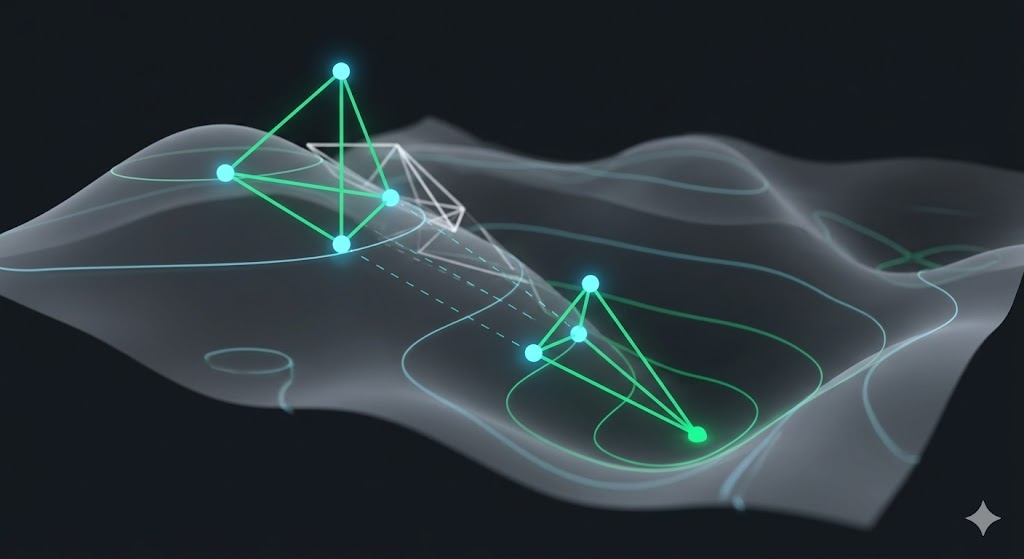
\includegraphics[width=\textwidth]{Imagenes/NelderMeadVisual.png}
        \end{center}
        
        \vspace{-0.3cm}
        \begin{center}
            \tiny \textcolor{gray}{
            Representación conceptual del simplex iterando sobre la topografía del error.
            }
        \end{center}

    \end{columns}

\end{frame}